\chapter{Reconstruction-based outlier detection}
\label{chap:reconstruction-detection}

%In this chapter the setup of this research is explained. First, the research directions and objectives are discussed in section \ref{sec:research_overview}. Second, we explain the baseline chosen for comparisons throughout this thesis. Finally, section \ref{sec:analysis_methodology} describes the data used for experimental evaluations and the performance metrics considered to assess our method.
%
%\section{Research challenges and questions}
%\label{sec:research_overview}
%- Can we improve a conventional on-line method approximating the principal components? And if so, for what cases does using random projections make a positive difference?\\
%- Can we exploit the randomness property of the projection matrices?\\
%
%The first Applying the in two ways, as reconstruction based method and feature reduction method.\\
%
%The second question will be answered by investigating the benefits of distributing the computations over several subsets of time series. Each base detector will have less information to derive its hypothesize concerning the outlierness of a data point, however, we expect that spreading our chances on different matrices (and possibly subsets) . This would also lead to a possibly beneficial setup as distributed systems are desired in many practical situations (example or citation!).\\
%
%
%List some `high-level' things that we want to achieve, not quantized yet!

\section{Data models, reconstructions and outlier scores}
[Clearly distinguish how we can get a model, but at least we are reconstructing from that model! Look at the figure here to see if PROJECTION shouldn't be MODELLING or something ]

\begin{figure}[h]
	\centering
	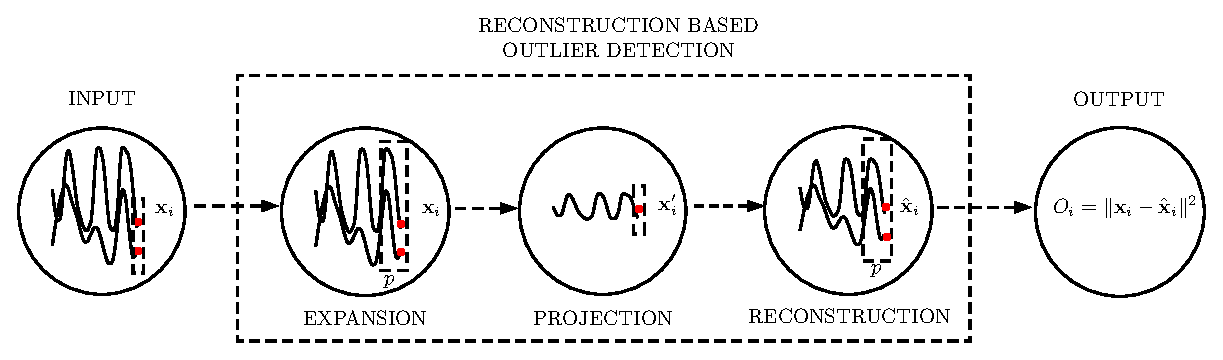
\includegraphics[scale=0.77]{research-design/reconstruction_outlierdetection}
	\caption{Reconstruction based outlier detection}
	\label{fig:researchdesign_reconstruction}
\end{figure}


% HOW WE DEFINE OUR OUTLIERS: RECONSTRUCTION ERROR + THRESHOLD




\section{Reconstruction-based methods for outlier detection in multivariate time series}

Look at section High-Dimensional Outlier Detection: Subspace method. AGGARWAL!!!!!!!!!!


\subsection{Auto-encoders}


\subsection{Autoregressive models}


\subsection{Principal component analysis}

Linear projections.\\

Examples:\\
Look at the paper from Numenta and University Pittsburgh.
PCA based approaches Robust PCA, osPCA (also in the THESIS folder paper).
Also the not yet published work by CMU.\\


What is it: discarding $d - k$ directions that have the smallest eigenvalues, i.e. the smallest variance. This way we obtain a model of the principal behavior of the data at hand.\\

If there's much correlation among the $d$ time series, $k$ is expected to be small, as it takes less components to capture the principal behavior (SPIRIT). \\

The mathematical procedure, and give a general statement about the runtimes (though depending on the particular PCA method).\\

Properties.\\
Streaming PCA receives increasing attention in recent literature studies like \cite{balzano2018streaming}. This increased interest is caused by its objective to describe the principal behavior of multivariate time series in a lower dimensional feature space. \\


Model of the data obtained by projections in principal directions
Which modelling method often is used is Principal component analysis






\section{Online principal component approximation: SPIRIT}
\label{sec:methods_baseline}

[Explain that SPIRIT is a well-known method and known to be tractable in high-dimensional settings (Aggarwal), and we are looking for high dimensional approaches, why Random projections?! How did we get there? It's data-independent making it very fast.]\\

SPIRIT is taken as the baseline method which is used to interpret the performance of the proposed methods under study in comparison to a commonly used method.

More detailed explanation and algorithm, but also visualize the update of the weights.\\

RUNTIME.\\

Downsides of using the principal component approximation is that it relies heavily on the forgetting factor and variance bounds. 
Therefore, an advantage of random projections is that it relies on nothing but the target dimensionality, which was seen to have little effect on the performance from some point.\\

SPIRIT is used as a baseline but also to find outliers in our feature reduction space, which then will be compared to SPIRIT in the original space.\\




\section{Open challenges}
Inaccurate?, speed-up?, memory intensive, sensitive to changes, and some parameters needed (not very critical though)
